\begin{figure*}[t]
    \centering
    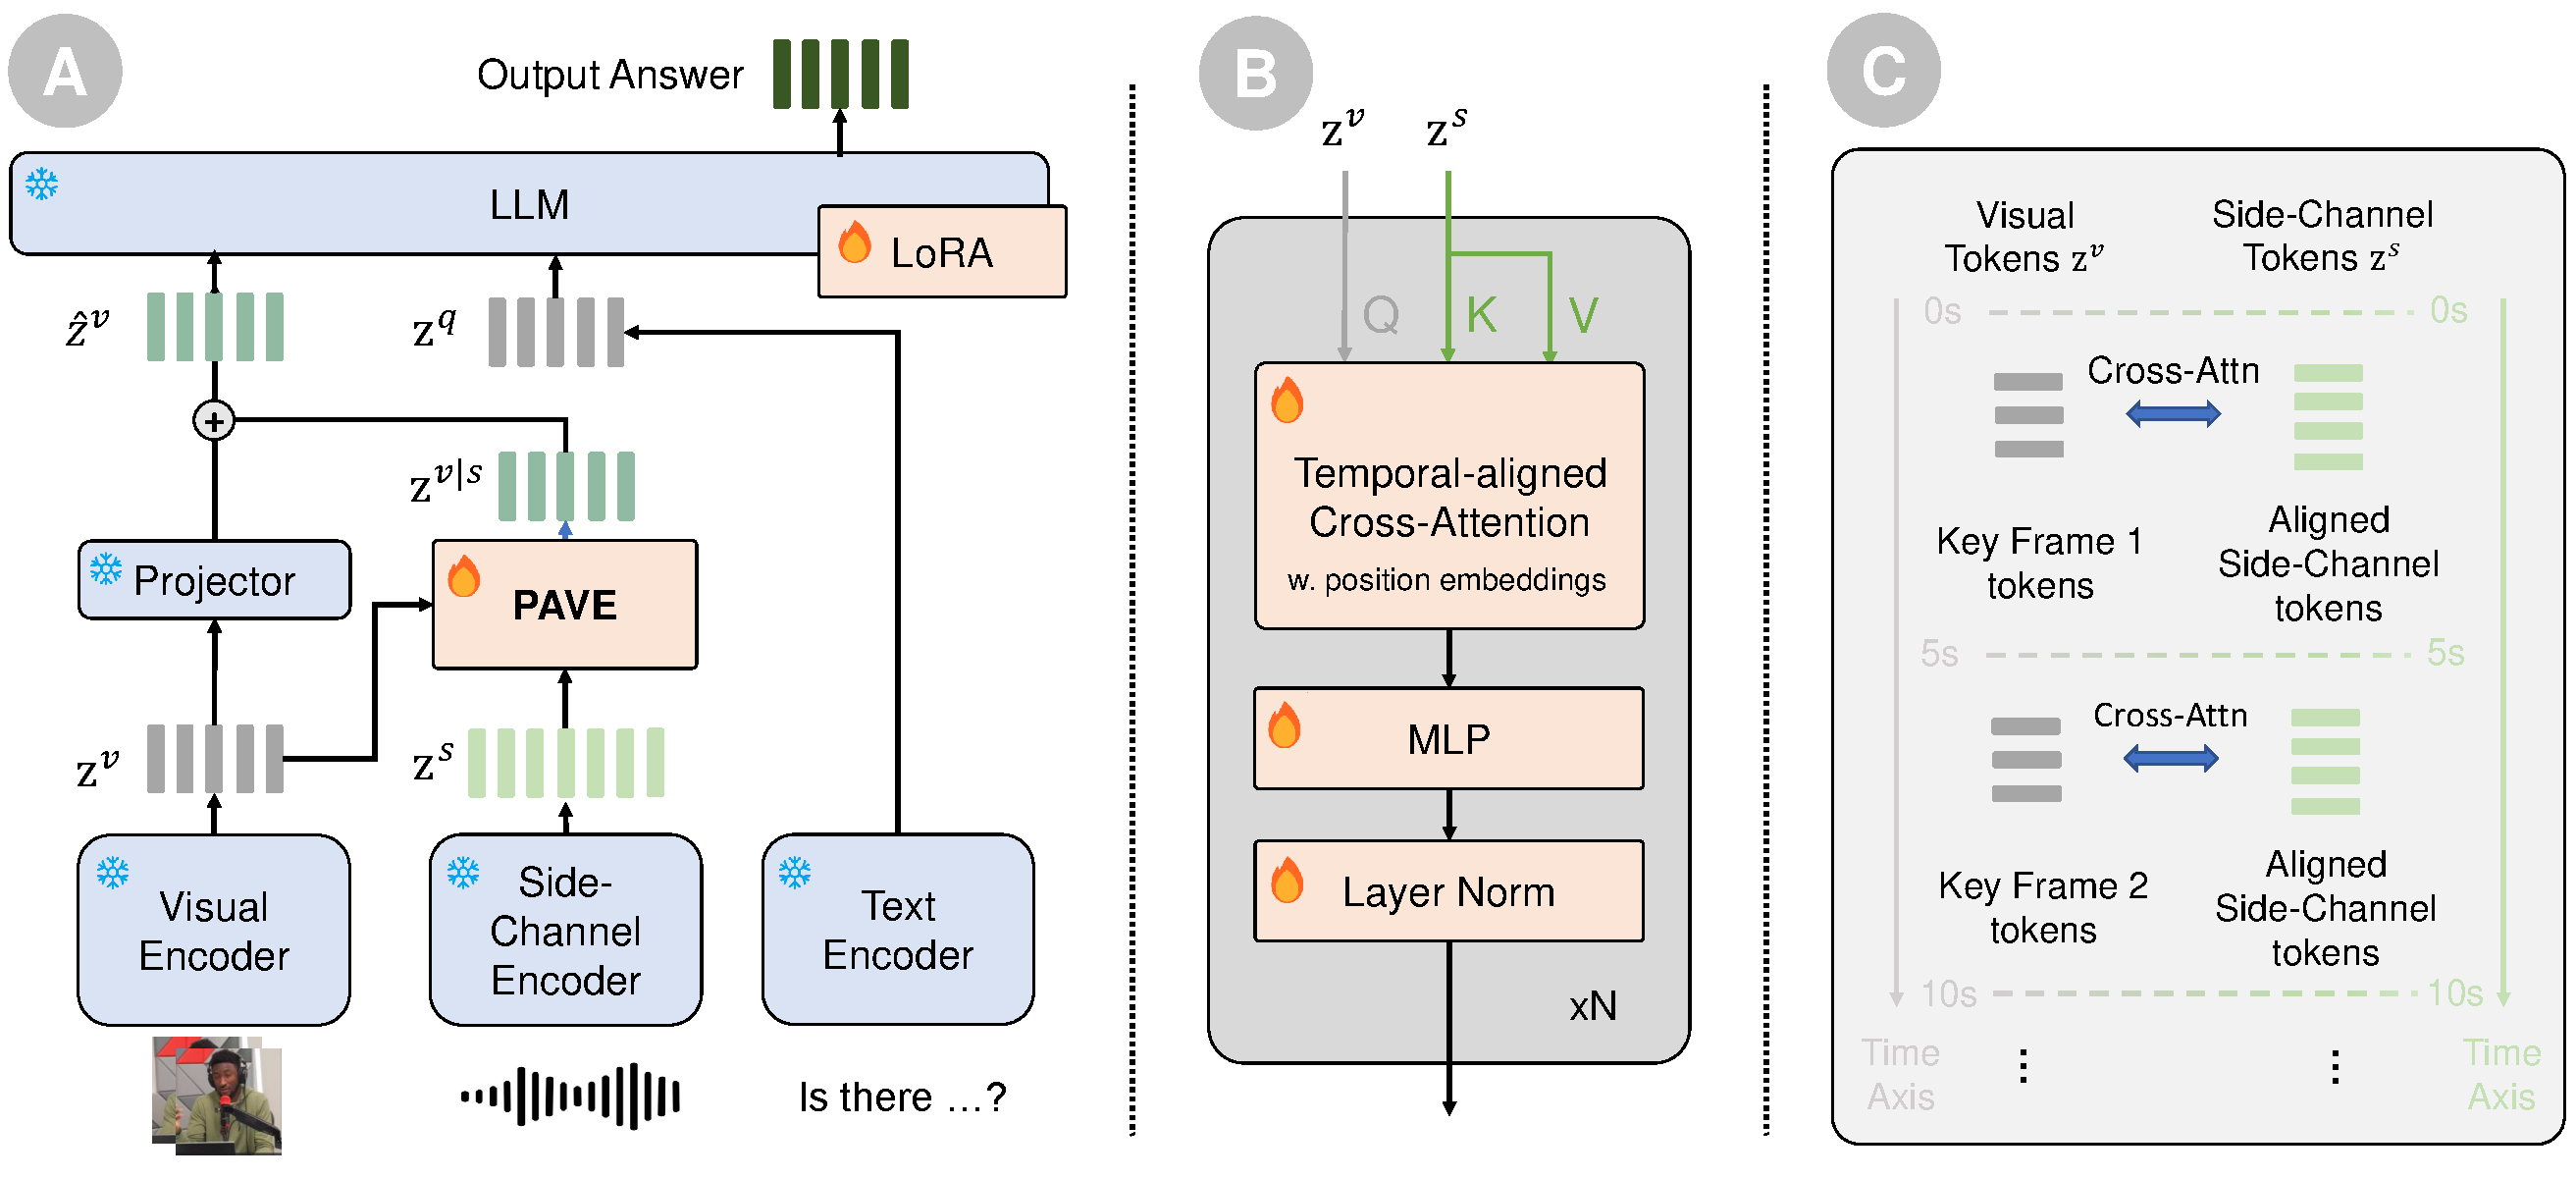
\includegraphics[width=0.85\linewidth]{new_figure_source/pave_overview_updated.pdf}
    \vspace{-0.5em}
    \caption{(a) \textbf{Overview of PAVE}. PAVE presents a simple, parameter-efficient adapter to integrate videos and side-channel signals. This is done by fusing side-channel tokens $\mathbf{z}^s$ and video tokens $\mathbf{z}^v$, and further adding the results to the original video tokens $\mathbf{z}^v$.  (b) \textbf{Details of PAVE's fusion function}. The fusion function $g(\cdot)$ consists of a few blocks of temporal-aligned cross-attention layer, MLP, and layer normalization. (c) \textbf{Temporal-aligned Cross-Attention}. Visual tokens $\mathbf{z}^v$ and side-channel tokens $\mathbf{z}^s$ are aligned along the temporal axis. A video token $\mathbf{z}^v(k)$ is treated as query, and only attends to keys and values (defined by side-channel tokens) in its temporal neighborhood.}
    \label{fig:structure_overview}
    \vspace{-1em}
\end{figure*}

\section{Patching and Adapting Video LLMs}
\label{sec:method}

% ovewview paragraph
We propose \textbf{PAVE}, a framework for adapting pre-trained Video LLMs to downstream tasks with side-channel signals. The key to our solution lies in a parameter-efficient, lightweight adapter, referred to as a patch. 
%only introduces a small number of parameters and operations and 
This patch fuses side-channel signals with the original visual tokens and updates them (see Figure~\ref{fig:structure_overview} (a)), and adds a LoRA module~\cite{hu2021loralowrankadaptationlarge} to the LLM, enabling efficient adaptation with a small number of parameters and operations and without altering the base model. 
%Additionally, we fine-tune the LLM using LoRA~\cite{hu2021loralowrankadaptationlarge}, enabling efficient adaptation through patching.
% ---
In what follows, we introduce the background on Video LLM, outline our problem formulation, and present our approach.
%and further describe the implementation details.   

%we present \textbf{PAVE}, a framework designed to \underline{P}atch and \underline{A}dapt \underline{V}id\underline{e}o LLMs. PAVE leverages a variant of cross-attention mechanism that operates between tokens derived from key video frames (as queries) and tokens from side-channel signals (as keys and values). This operations seeks to align the video frames and side-channel signals along the time axis, fuse the signals from both sources, and then update the input visual tokens to the LLM. In doing so, PAVE allows for the input of supplementary signals, and introduces a small number of parameters and operations with a negligible memory footprint and computing cost, while enabling effective adaptation to various downstream tasks without altering pre-trained models.


\subsection{Preliminaries: Video LLM}
A Video LLM takes a video $\mathbf{X}^v$ and a text query $\mathbf{X}^q=\{x^q\}$ as input, then generates a text answer $\mathbf{X}^a=\{x^a\}$. We assume that $\mathbf{X}^v = \{\mathbf{X}^v_1, \mathbf{X}^v_2, ..., \mathbf{X}^v_K\}$, \ie, a video is represented by $K$ key frames, where $K$ may vary across videos. $\mathbf{X}^v$ is first encoded by a visual encoder
% (including the vision backbone and its projector) 
$h_v(\cdot)$ into a set of visual tokens $\{\mathbf{z}^v(k) \in \mathbb{R}^{M \times d}\}$, where $\mathbf{z}^v(k)$ indicates $M$ tokens encoded from the $k$-th key frame within the video ($k \in [1, K]$). Similarly, $\mathbf{X}^q$ is processed by a text encoder $h_t(\cdot)$, which embeds individual words $x^q$ into text tokens $\{\mathbf{z}^q \in \mathbb{R}^d\}$ with $\mathbf{z}^q = h_t(x^q) $. 
These tokens are further combined and processed by an LLM $f(\cdot)$ that decodes $\mathbf{X}^a$ in an autoregressive manner
\begin{equation}
    f\left( \left[ \{\mathbf{z}^v(k)\}, \{\mathbf{z}^q\}, \{\mathbf{z}^a_{<i}\} \right]; \mathbf{\theta} \right) \rightarrow x_i^a, \label{eq:llm}
\end{equation}
where $\{\mathbf{z}^a_{<i}\}$ are text tokens from previously generated answer $x^a_{<i}$, \ie, $\mathbf{z}^a = h_t(x^a)$. $\mathbf{\theta}$ denotes LLM parameters. 

\subsection{Video Tasks with Side-Channel Signals}
% problem formulation / use cases
We consider adapting a pre-trained Video LLM to downstream tasks with side-channel signals $\mathbf{X}^s$. Similar to videos, we assume that $\mathbf{X}^s = \{\mathbf{X}^s_1, \mathbf{X}^s_2, ..., \mathbf{X}^s_{K_s}\}$, \ie, the side-channel signals also follow a temporal order and are split into $K_s$ blocks. We additionally assume a separate encoder (with possible projector) $h_s(\cdot)$ to process $\mathbf{X}^s$ into a collection of tokens $\{\mathbf{z}^s(k_s) \in \mathbb{R}^{M' \times d} \}$, where $\mathbf{z}^s(k_s)$ is $M'$ tokens encoded from the $k_s$-th block of the side-channel.  It is worth noting that this formulation encapsulates a range of video tasks. We describe some of these tasks considered in our experiments. 

\begin{itemize}
    \item \textbf{Audio-visual understanding}. This task requires jointly processing video and its accompanying audio data (as side-channel signals) for scene understanding, such as event recognition~\cite{xiao2020audiovisual} or QA~\cite{alamri2019audiovisualsceneawaredialog}. 
    \item \textbf{3D scene understanding}. This task focuses on reasoning about the 3D scene using a video of a 3D scan~\cite{azuma_2022_CVPR}. Camera trajectories, as well as an optional sequence of depth maps, constitute the side-channel signals.  
    \item \textbf{Multi-view video understanding}. This task involves combining multi-view videos for visual recognition, \eg, using exocentric videos to complement egocentric video for understanding human activities~\cite{grauman2024ego}. 
    \item \textbf{Enhancing video representations}. This task seeks to enhance the visual representation in the Video LLM. This is done by integrating low resolution, high frame rate frames with the original input of high resolution, low frame rate frames, following the key idea of SlowFast networks~\cite{feichtenhofer2019slowfastnetworksvideorecognition}.

\end{itemize}

\subsection{Our Design of PAVE}
% the key idea: x-attention for fusion and summation for aggregation; technical details about temporal alignment / positional encoding

Our goal is to integrate side-channel signals $\mathbf{X}^s$ into the LLM to enhance video reasoning, without modifying the structure of $f(\cdot)$ and encoders ($h_v(\cdot)$ and $h_t(\cdot)$), nor adding any major set of parameters. To achieve this goal, our key idea is learning a function $g(\cdot)$ to fuse side-channel tokens $\{\mathbf{z}^s(k_s)\}$ with the original visual tokens $\{\mathbf{z}^v(k)\}$. The fusion results have the same size of $\{\mathbf{z}^v(k)\}$, and will be further used to update $\{\mathbf{z}^v(k)\}$. Formally, our design of PAVE, as shown in Figure~\ref{fig:structure_overview} (a), is expressed as
\begin{equation}
\begin{split}
    \text{fusion:} \quad & \{\mathbf{z}^{v|s}(k)\} = g([\{\mathbf{z}^s(k_s)\}, \{\mathbf{z}^v(k)\}]; \phi)\\
    \text{summation:} \quad & \mathbf{\hat{z}}^{v}(k) = \mathbf{z}^{v}(k) + \mathbf{z}^{v|s}(k),
\end{split}\label{eq:pave}
\end{equation}
where $\phi$ denotes learnable parameters of $g(\cdot)$. 

Intuitively, $g(\cdot)$ injects side-channel information into a set of tokens of the same size as the original visual tokens, based on which a simple summation can be performed to form a residual connection. A key feature of this design is that the number of input tokens to $f(\cdot)$ remains unchanged. As the main computational cost lies in $f(\cdot)$, doing so results in a negligible overhead. 

\medskip
\noindent \textbf{The fusion function $g(\cdot)$}. Our fusion function is realized using a variant of cross-attention, as illustrated in Figure~\ref{fig:structure_overview} (b). Specifically, the vision tokens $\{\mathbf{z}^v(k)\}$ are transformed into the queries, and the side-channel tokens $\{\mathbf{z}^s(k_s)\}$ form the keys and values. To align video and side-channel signals in time while maintaining a low computation cost, we consider a local cross-attention, named temporal-aligned cross-attention, where a query $\mathbf{z}^v(k)$ only attends to keys and values in its temporal neighborhood, \ie, $\{\mathbf{z}^s(k_s)\}$ with $k_s \in N(k)$ (see Figure~\ref{fig:structure_overview} (c)). Before computing the cross attention, rotary positional embeddings~\cite{su2024roformer} are added to the queries and keys. After cross attention, an MLP with layer normalization is applied to further transform the features, similar to a standard Transformer block~\cite{vaswani2017attention}.


\medskip
\noindent \textbf{Integration with LoRA and training loss}. We further combine PAVE with LoRA~\cite{hu2021loralowrankadaptationlarge} by adding a small set of parameters in the form of low rank approximation $\Delta \theta$ to the LLM $f(\cdot)$. Putting things together, PAVE minimizes the standard negative log likelihood of its output when adapting to a downstream task. This is given by 
\begin{equation*}
\argmin_{\mathbf{\Delta\theta}, \mathbf{\phi}} \ \mathbb{E}_{\mathcal{D}} \ \left[ -\log p \left( x^a_i | \left[ \{\mathbf{\hat{z}}^{v}\}, \{\mathbf{z}^{q}\}, \{\mathbf{z}^a_{<i}\} \right]; \theta+\Delta \theta, \phi \right) \right],
\end{equation*}
where $\mathcal{D}$ is the data distribution approximated by the training set $(\mathbf{X}^v, \mathbf{X}^q, \mathbf{X}^a) \sim \mathcal{D}$. $\{\mathbf{\hat{z}}^{v}\}$ is computed using Eq.\ \ref{eq:pave}, thus creating a dependency on $g(\cdot)$ and its parameters $\phi$.
%The learnable parameters thus include the LoRA parameters $\Delta \theta$ in $f(\cdot)$, and the parameters $\phi$ in $g(\cdot)$ 

%A simple solution is given by LoRA~\cite{hu2021loralowrankadaptationlarge}. It learns a small set of parameters in the form of low rank approximation $\Delta \theta$. However, this solution does not allow us to make use of $\mathbf{X}^s$. 

% \subsection{Implementation Details}
% % all other things including some of the implementation details.
% Inside the attention layer, we add rotary position embedding to the query and key tokens. Specifically, we apply different rotary positional embedding according to the layout of side-channel tokens $\mathbf{z}^s$. We mainly consider two types of $\mathbf{z}^s$: (a) $\{\mathbf{z}^s\}$ includes both spatial and temporal dimensions, such as tokens from video backbones or from 3D backbone; and (b) $\{\mathbf{z}^s\}$ only contains temporal dimension, such as audio tokens. For the first case, we will add 3D rotary positional embedding (along the temporal, height, and width dimensions). For the second case, we will only add rotary positional embedding along the temporal axis. After cross-attention, we use a two-layer MLP, followed by a layer norm. We initialize the $\gamma$ in the layer norms to zero. For all experiments, we use a learning rate of 2e-5 and a batch size of 32 to adapt the pre-trained Video LLM.


\begin{comment}
\subsection{Background}
Current video Large Language Models (Video LLMs) have three components: Visual Encoder, Projector, and Language Model (LM).

\noindent\textbf{Visual Encoder.} It encodes the vision input into a latent feature space. The common choices for the vision encoder are ViT\cite{dosovitskiy2021imageworth16x16words} from CLIP\cite{radford2021learningtransferablevisualmodels}, SigLIP \cite{zhai2023sigmoidlosslanguageimage}, and multi-modality encoder LanguageBind\cite{zhu2023languagebind}. The encoded feature will be delivered to the adapter. We call features from the vision encoder as original visual tokens, $V_{origin}$.


\noindent\textbf{Projector.} The projector is the module convert the vision feature to the text latent space. In many recent research\cite{tong2024cambrian1fullyopenvisioncentric, liu2024llavanext} shows that the 2 layers MLP is strong enough to bridge the domain gap. We name the feature converted by after the projector as projected visual tokens, $V_{projectored}$

\noindent\textbf{Language Model.} The language model will process projected vision information and the questions to give an answer. The popular choice for the language model are Llama\cite{touvron2023llama2openfoundation,llama3_2}, Vicuna\cite{vicuna2023}, and Qwen-2\cite{yang2024qwen2technicalreport}.


\subsection{PAVE structure}
The overview of the PAVE structure is shown on the left panel of figure~\ref{fig:structure_overview}. For specific downstream tasks, the high level idea of PAVE is to create a 'Patch' and attach it to the Video LLM without altering the original model parameters and adapt the Video LLM into a new setting. This patch collects the task-specific additional information and add it back to the adapted visual tokens $V_{adapted}$, using a residual connection. 

\noindent\textbf{Input of the PAVE.} PAVE’s input has two sources: original visual tokens, $V_{origin}$, from the Video LLM's vision encoder, and the other is task-specific tokens $T$ from the encoder which encode the task-specific additional information.

\noindent\textbf{Temporal Alignment Module}
Given the fact that, the task-specific tokens $T$ and original visual tokens $V_{origin}$ may have different temporal granularities. Considering that temporally close visual and additional information are strongly correlated, as they jointly represent the same scene, we use temporal alignment module to explicit align them. This approach not only reduces noise introduced by temporal misalignment but also further reduces computational resource needed in cross-attention.

To do this we first split the task-specific tokens $T$ and original visual tokens $V_{origin}$ based on their smallest temporal unit, respectively. We then have $T = \{T_0, T_1, ... , T_n\}$ and $V_{origin}=\{V_0, V_1, ... , V_m\}$. For instance, if input of the Video LLM's vision encoder consist of 32 frames, then original visual tokens $V_{origin}$ should be split into $\{V_0, V_1, ... , V_{31}\}$. We always use the $\{V_0, V_1, ... , V_m\}$ as anchors on the temporal axis and evenly divide the $\{T_0, T_1, ... , T_n\}$ into $m$ groups.


\begin{align*}
\{T_0, T_1, \dots, T_n\} &= \Big\{ \{T_{00}, T_{01}, \dots, T_{0k}\}, \\ 
                          &\quad \{T_{10}, T_{11}, \dots, T_{1k}\}, \dots, \\ 
                          &\quad \{T_{m0}, T_{m1}, \dots, T_{mk}\} \Big\}
\end{align*}


For some special case that $\{T_0, T_1, ... , T_n\}$ could not be evenly split into m groups, we will pad the group which lengthen is smaller than $\ceil*{\frac{n}{m}}$. Right panel of figure~\ref{fig:structure_overview} show the visualization of temporal alignment module. We then pair the $V_i$ with $\{T_{i0}, T_{i1}, \dots, T_{ik}\}$ as mini-batch $mbatch_i = (V_i, \{T_{i0}, T_{i1}, \dots, T_{ik}\})$ and create $m$ mini-batches in total.

\noindent\textbf{Cross-Attention Module and 3-dimension Rotary Positional Embedding.}
After Obtaining the $m$ mini-batches from the Temporal Alignment Module we conduct cross-attention within each mini-batch, Where $V_i$ will be the query and $\{T_{i0}, T_{i1}, \dots, T_{ik}\}$ will be the key. Thus it aggregate the additional information from $\{T_{i0}, T_{i1}, \dots, T_{ik}\}$ into $V_i$ and and yield a group of updated tokens $V_{updated}=\{V_{updated_0}, V_{updated_1}, ... , V_{updated_m}\}$

During the cross-attention, We mainly consider two types of task-specific tokens $T$ : 1. tokens $T$ with spatial dimensions, such as video tokens from video backbones and 3D tokens from 3D backbone, 2. tokens $T$ without spatial dimensions, such as audio tokens. For the first case we will add 3 dimension rotary positional embedding along the temporal, height and width dimension. For the second case we will only add rotary positional embedding along the temporal axis.

\noindent\textbf{Zero-Initialized Residual Connection.}  After aggregating all additional information into $V_{updated}$, $V_{updated}$ will pass through an MLP and a Layer Normalization layer. Specifically, we initialize the $\gamma$ in layer norm to zero, this will ensure that the beginning of the training PAVE module will not have any effect on the Video LLM. 
Finally we add up $V_{updated}$ with the projected visual tokens $V_{projected}$. The $V_{adaptored} = V_{updated} + V_{projected}$ will be sent into the LLM for reasoning.

\subsection{The Training of PAVE}
In the PAVE, the Cross-Attention layers, the MLP and the layer normalization layer are trainable, while other modules remain forzen. During the adaptation, we also apply LoRA to the LLM to adapt the LLM for making use of the additional information.
We use the original auto-regressive training objective to train the PAVE, specially for a sequence of length L, we maximize the probability of the target answers $\mathbf{X}_\text{a}$ during the adaptation by:
\begin{align*}
        p(\mathbf{X}_\text{a} \mid V_{adaptored}, \mathbf{X}_\text{instruct}) = \\
    \prod_{i=1}^{L} p_\theta (x_i \mid V_{adaptored}, \mathbf{X}_\text{instruct, $<$ i}, \mathbf{X}_\text{a, $<$ i})
\end{align*}
where, the $\mathbf{X}_\text{a}$ is the target answer, $V_{adaptored}$ is the PAVE adapted visual features, $\mathbf{X}_\text{instruct}$ is the question and instruction, and $\theta$ represent the all trainable parameters.
\end{comment}